\documentclass[article,shortnames]{jss}
%%%%%%%%%%%%%%%%%%%%%%%%%%%%%%
%% declarations for jss.cls %%%%%%%%%%%%%%%%%%%%%%%%%%%%%%%%%%%%%%%%%%
%%%%%%%%%%%%%%%%%%%%%%%%%%%%%%

\usepackage{amssymb}
%% almost as usual
\author{Stefan R\"odiger$^{\ddag,\S}$\\Lausitz University of\\Applied Sciences\\ \& Charit\'e
	\And Thomas Friedrichsmeier$^{\ddag,\S}$\\Ruhr-University Bochum
	\AND Prasenjit Kapat\\The Ohio State University
	\And Meik Michalke\\Heinrich Heine University\\D\"usseldorf
}
\title{\pkg{RKWard} -- A Comprehensive Graphical User Interface and Integrated Development Environment for Statistical Analysis with \proglang{R}}

%% for pretty printing and a nice hypersummary also set:
\Plainauthor{Stefan R\"odiger, Thomas Friedrichsmeier, Prasenjit Kapat, Meik Michalke} %% comma-separated
\Plaintitle{RKWard -- A Comprehensive Graphical User Interface and Integrated Development Environment for Statistical Analysis with {R}} %% without formatting
\Shorttitle{\pkg{RKWard} a GUI for \proglang{R}} %% a short title (if necessary)

%% an abstract and keywords
\Abstract{
  \proglang{R} is a free open-source implementation of the \proglang{S} statistical computing
language and programming environment. The current status of \proglang{R} is a
command line driven interface with no advanced cross-platform graphical user
interface (GUI), but it includes tools for building such. Over the past
years, proprietary and non-proprietary GUI solutions have emerged, 
based on internal or external tool kits, with different scopes and technological concepts.
For example, \proglang{Rgui.exe} and \proglang{Rgui.app} have
become the de facto GUI on the Microsoft Windows and Mac OS X platforms, respectively, for most users. 
In this paper we discuss \pkg{RKWard} which aims to be both a
comprehensive GUI and an integrated development environment 
for \proglang{R}. \pkg{RKWard} is based on the \pkg{KDE} software libraries. Statistical
procedures and plots are implemented using an extendable plugin
architecture based on \proglang{ECMAScript} (\proglang{JavaScript}), \proglang{R}, and XML. \pkg{RKWard}
provides an excellent tool to manage different types of data objects;
even allowing for seamless editing of certain types. The objective of
\pkg{RKWard} is to provide a portable and extensible \proglang{R} interface for both
basic and advanced statistical and graphical analysis, while not
compromising on flexibility and modularity of the \proglang{R} programming
environment itself.

\line(1,0){40}
\item$^{\ddag}$Equal contribution, $^{\S}$Corresponding authors
%%
}
\Keywords{GUI, integrated development environment, plugin, \proglang{R}}

\Plainkeywords{GUI, integrated development environment, plugin, R} %% without formatting
%% at \leftarrowst one keyword must be supplied

%% publication information
%% NOTE: Typically, this can be left commented and will be filled out by the technical editor
%% \Volume{13}
%% \Issue{9}
%% \Month{September}
%% \Year{2004}
%% \Submitdate{2004-09-29}
%% \Acceptdate{2004-09-29}

%% The address of (at least) one author should be given
%% in the following format:
\Address{
  Stefan R\"odiger\\
  Lausitz University of Applied Sciences\\
  Department of Bio-, Chemistry and Process Engineering\\
  AND\\
  Center for Cardiovascular Research (CCR)\\
  Charit\'e, Germany\\
  E-mail: \email{stefan\_roediger@gmx.de}\\
  E-mail: \email{rkward-devel@lists.sourceforge.net}\\
}

% \Address{
%  Prasenjit Kapat\\
%  Affiliation\\
%  Department\\
%  E-mail: \email{noname@here.org}
% }
% \Address{
%  Meik Michalke\\
%  Affiliation\\
%  Department\\
% }


%% for those who use Sweave please include the following line (with % symbols):
%% need no \usepackage{Sweave.sty}

%% end of declarations %%%%%%%%%%%%%%%%%%%%%%%%%%%%%%%%%%%%%%%%%%%%%%%

\begin{document}

%% include your article here, just as usual
%% Note that you should use the \pkg{}, \proglang{} and \code{} commands.

% !TEX root = RKWard_paper.tex
\section{Background and motivation}
\label{background}
In mid 1993 Ihaka and Gentleman published initial efforts on the computing
language and programming environment \proglang{R} on the \emph{s-news} mailing list. Ambitions for
this project were to develop an \proglang{S}-like language without inheriting memory
and performance issues. The source code of \proglang{R} was finally released in 1995, and 
since 1997 development has evolved under the umbrella of the \proglang{R} 
Development Core Team \citep{RDCT2001, RDCT2010, Ihaka_Gentlemen_1993}.
\proglang{R} does not include an advanced cross-platform graphical user interface (GUI) as known from other
statistical software packages. However, \proglang{R} includes tools for building GUIs
mainly based on \proglang{Tlc/Tk} \citep{Dalgaard2001, Dalgaard2002}. Meanwhile a
plethora of \proglang{R} GUIs have emerged (see \url{http://www.sciviews.org/_rgui/} for a
comprehensive list). In 2005 John Fox released version 1.0 of \proglang{R} Commander (package \pkg{Rcmdr}), which
can be considered a milestone in \proglang{R} GUI development; it was the first GUI
implementation that was able to make statistical tests,
plots and data manipulation easily accessible for \proglang{R} novices.
John Fox stated that \pkg{Rcmdr}'s target was to provide
functionality for basic-statistical courses, though the features have increased over
time beyond this \citep{Fox2005, Fox2007}. In November 2002 Thomas Friedrichsmeier
started the \pkg{RKWard} open-source software project with the goal to create a GUI for
\proglang{R} based on \pkg{KDE}\footnote{\url{http://www.kde.org/}} and \pkg{Qt}\footnote{\url{http://qt.nokia.com/}} technologies.

The scope of \pkg{RKWard} is deliberately broad, targeting both \proglang{R} novices and experts.
For the first group, the aim is to allow any person with knowledge on
statistical procedures to start using \pkg{RKWard} for their everyday work 
without having to learn anything about the \proglang{R} programming language,
at least initially. At the same time, \pkg{RKWard} tries to support users who want to learn and
exploit the full flexibility of the \proglang{R} language for automating or customizing
an analysis. At the other end of the learning curve, \pkg{RKWard} provides advanced integrated development environment (IDE)
features to \proglang{R} experts to assist in writing \proglang{R} scripts. Yet, the idea
is that \proglang{R} experts too will benefit from the availability of task-oriented GUI
dialogs, such as when exploring an unfamiliar type of analysis
or by allowing to implement routinely performed tasks as a GUI element. In
addition, many features like the integrated data editor and the plot preview 
will be useful to \proglang{R} novices and \proglang{R} experts alike in their everyday work
(see Section~\ref{sec:user_interface}).

\pkg{RKWard} provides a high level of transparency about the steps that are needed to
perform any supported task in \proglang{R}, in order to make it easy for the user to see
complete codes for all GUI actions\footnote{
  This distinguishes \pkg{RKWard} from \proglang{R} GUIs such as \pkg{Red-R} (\url{http://www.red-r.org/}), which 
  specifically aims to hide the complexities of the \proglang{R} programming language, following the concept of visual data-flow 
  programming \citep{Sutherland1966}. In contrast, \pkg{RKWard} limits itself to generate \proglang{R} code from GUI settings.
}. In doing so, \pkg{RKWard} deliberately generates
comparatively verbose code. It avoids wrapping complex sequences of data
manipulation or analysis into custom high-level \proglang{R} functions. The task of
providing high-level functions is logically independent of the development of the
GUI frontend, and should best be addressed in dedicated \proglang{R} packages, where necessary.
This approach allows to make better use of the modular design of \proglang{R}, avoids
locking-in users to a specific GUI application, and provides them with more options for
customizing the generated code patterns.

While \pkg{RKWard} tries to address users wishing to learn \proglang{R}, it is specifically not
designed as a teaching tool (such as \pkg{Rcmdr} or \pkg{TeachingDemos}), but as
a productive tool. Dialogs for statistical procedures in \pkg{RKWard} do not
necessarily show a one-to-one correspondence to the underlying steps in \proglang{R}, but are
rather oriented at statistical tasks. Furthermore, \pkg{RKWard} does not impose
artificial limitations on how users can work with the application. For example,
the user is not limited to using only one \code{data.frame} or one model at a
time. \pkg{RKWard} is designed to allow users to create custom GUI dialogs
easily (see Sections~\ref{sec:technical_plugins} and \ref{sec:example_plugin}).

\pkg{RKWard} is licensed under the terms of the GNU General Public License Version 2
or higher. However, due to its dependencies, \pkg{RKWard} binaries are effectively
distributable only under the terms of Version 2 of the license. Parts of the documentation are available under the
GNU Free Documentation License. While the project remains in constant development, a growing
number of users employs \pkg{RKWard} in productive scenarios. The source code,
selected binaries and documentation is hosted at SourceForge
(\url{http://rkward.sourceforge.net/}). Selected key milestones of the development of \pkg{RKWard} are
visualized in Figure~\ref{fig:timeline}.

\begin{figure}[t!]
 \centering
 \includegraphics[clip=true,trim=0cm 5.7cm 0cm 5.7cm,width=16cm]{../figures/timeline.pdf}
 \caption{Timeline of important development milestones and changes in \pkg{RKWard}.
          Time is presented on an arbitrary scale. Here \pkg{Qt}3 and \pkg{Qt}4 refers to the 3.x and
          4.x versions of the \pkg{Qt} libraries, respectively and \pkg{KDE}4 refers to the
          4.x version of the \pkg{KDE} libraries.}
 \label{fig:timeline}
\end{figure}

In this paper we will first give an overview over the main GUI elements and
features of \pkg{RKWard} (Section~\ref{sec:user_interface}), followed by a short example 
of a simple \pkg{RKWard} session (Section~\ref{sec:using_RKWard}). Next, technical 
details of the implementation will be discussed, comparing them briefly to 
competing GUI solutions, where appropriate (Section~\ref{sec:technical}).
Finally, we show an example for creating a plugin extension to \pkg{RKWard} 
(Section~\ref{sec:example_plugin}).

\section{Installing and Starting RKWard}
\label{sec:installing_starting_RKWard}
RKWard can be downloaded free of charge in source and binary from
\url{http://sourceforge.net/}. On the GNU/Linux
platform, binary packages are available for many major distributions,
including Debian, Ubuntu, OpenSuse, Gentoo, and Fedora. On the Windows
platform, RKWard is available in two forms: as a single binary
installer (requires existing installations of
\proglang{R} and \proglang{KDE}) and
as an installation bundle (including \proglang{R} and
essential parts \proglang{KDE} SC). At the time of
this writing, the developers lack the resources to support a MacOS X
port, and especially to provide binaries for MacOS X. However, RKWard
has been shown to be compilable and installable on the Mac, and appears
to be mostly functional.

RKWard cannot be loaded from within an \proglang{R}
session, but rather it is started as a stand-alone application with an
embedded \proglang{R} engine. To facilitate the first
steps for new users, a dialog offers the choice to load an existing
workspace, to start with an empty workspace, or to create a new
data.frame and open that for editing. Also, an overview help-page is
shown in the document area of the main window. Both start-up features
can be turned off.
\section{Main elements of the user interface}
\label{sec:user_interface}
This section gives an overview of the main user interface elements and features of RKWard.
For a use-case oriented example of an RKWard session, see Section~\ref{sec:using_RKWard}.

The default layout of the main application window is divided into five
parts, as depicted in Figure~\ref{fig:main_window}. While many aspects
of the GUI can be customized by the user, for simplicity we will
describe the default appearance of RKWard in the present section. The
top of the window is occupied by menu bar and toolbar (Figure~
\ref{fig:main_window}A). The content of both bars is partially context
sensitive, e.g., the Edit menu will offer
one set of actions when the current document window is a data editor,
and another set of actions for an \proglang{R} script
editor window. To ease orientation, all top level menus remain
persistent, even if no actions are available for that menu in the
current context. The menu bar of the main window is also the central
access point to most data import, manipulation, analysis and
visualization features (see Section~\ref{sec:analyzing_data}) for which RKWard provides a GUI
interface.

A status bar is shown at the bottom of the window. This contains (from
right to left) an indication of the status of the
\proglang{R} engine (busy or idle), a display of the
current working directory, and a multi purpose region which is used to
display additional information on some menu items and other GUI
elements, when hovering the mouse pointer over them.

The central area is divided into a document view area
(Figure~\ref{fig:main_window}C) and two panel subwindows
(Figure~\ref{fig:main_window}B and D). The panels can be resized or moved to
another edge of the central area, independently. All panels can be
toggled by mouse or keyboard shortcuts. When a panel is closed, the
document view area (see below) is automatically re-sized to take up the
free space.

\begin{figure}[htp]
 \centering
 \includegraphics[width=15.446cm,height=10.949cm]{../figures/main_window.png}
 \caption{Default RKWard main window after start up. 
A) Menu bar, B) navigator element, C) editor, output, 
and data management. D) embedded \proglang{R} console. 
E) In addition to the menu bar at the top A) toolbar buttons 
on the bottom of the main window give quick access to the command log, 
running jobs, an \proglang{R} console, and the \proglang{R} help. 
RKWard main window. Panels B) and D) can be resized or collapsed. The navigator element B)
presents detailed information (e.g. type, class) about objects and their properties.}
 \label{fig:main_window}
\end{figure}

The left panel contains the file browser (see Section~\ref{sec:further_tool_windows}) and the
workspace browser (see Section~\ref{sec:workspace_browser_object_viewer}), by default. The
bottom panel contains the tool windows, namely, Command
log (Section~\ref{sec:further_tool_windows}), Pending Jobs (Section~\ref{sec:further_tool_windows}), \proglang{R} Console
(Section~\ref{sec:using_R_console}), and Help Search (Section~\ref{sec:help_system}).

The remainder of the central area is a single row TDI (Tab document
interface) for different documents. Currently, the supported types of
documents are results output (Section~\ref{sec:results_output}), spreadsheet-like data editors
(Section~\ref{sec:spreadsheet}), help pages (Section~\ref{sec:help_system}), script editors (Section~\ref{sec:code_editor}),
object summaries (Section \ref{sec:workspace_browser_object_viewer}), and also
\proglang{R} onscreen graphics devices (Section~\ref{sec:technical_graphics}). Early uses of TDIs date back to 1988 and are
widely applied nowadays \citep{Hopkins2005, MDN2010,
KimLutteroth2010}. The order of tabs can be conveniently re-arranged
using drag and drop.

Both document windows, and tool views, can be detached from the main
window as independent windows managed by the window manager, and also
re-attached. This feature allows to work with multiple documents, e.g.,
scripts or data editors at the same time, conveniently. On{}-screen
graphics device windows are created detached by default, but can also
be attached to the document view area of the main window.

Windows can be shown (or activated) using a mouse device with point and
click, as well as using a series of keyboard shortcuts (defined by
default) for switching between the different tool and document windows.
Key bindings can be configured from the GUI via "Settings->Configure Shortcuts". 
However, for technical reasons, only the shortcuts of those
components currently active will be listed. Thus, for example, to
configure data editor shortcuts one has to open a data editor first and
then to select ``Settings->Configure Shortcuts''. Since RKWard relies on
\proglang{KDE} SC editor component as editor component
shortcuts for the script editor (Section~\ref{sec:code_editor}) are managed separately using
``Settings->Configure Editor->Shortcuts''. On most systems, it is also
possible to configure shortcuts by right-clicking on the respective
menu item.

The choice of actions which are available on the tool bar can be
configured via ``Settings->Configure Toolbars``. Further, it is possible to add and remove sets
of data manipulation and analysis features from the GUI using
''Settings->Configure RKWard/Plugins``.

\subsection{Workspace browser and object viewer}
\label{sec:workspace_browser_object_viewer}

The workspace browser allows to view
and manipulate \proglang{R} objects, somewhat similar
to a regular file-system browser. This includes both user objects
(data, functions) in the \code{.GlobalEnv}, and in other environments on the
\proglang{R} search path (typically
\proglang{R} package environments). Objects are shown
in a hierarchical tree structure. For instance, an object of class
list can be expanded to show the objects
contained inside the list, by clicking on a
+-symbol to the left of the object name.
The basic type of each object is visualized by different icons. Further
information on each object can be obtained by hovering the mouse
pointer over the respective icon. This will display a tooltip window,
including information such as dimensionality or function arguments,
depending on the type of object. Objects inside the \code{.GlobalEnv} can be
removed, renamed, and edited from the context menu.

Literally hundreds or even thousands of objects are present in a typical
\proglang{R} session. This can be overwhelming at
first, therefore the workspace browser offers to show only a certain
subset of objects, e.g. only functions or only data objects, including
or excluding hidden objects (with names
starting with a 
``.''), or showing only the contents of \code{.GlobalEnv} as
opposed to all environments on the search path.

Several actions are available from the context menu (by right-clicking
on one of the objects), however some of these actions are only
available for some types of objects. These allow to search the
\proglang{R} help for information on that object, to
open a window with detailed information about the object, to delete, rename or copy the object to a new symbol name, or to
copy it to the \code{.GlobalEnv}. Further the context menu allows to open
supported types of objects for editing (see Section~\ref{sec:spreadsheet}; currently, only
\code{data.frame}s can be edited, and only when inside the \code{.GlobalEnv}). 

An object list similar to the workspace browser (but showing only the
globalenv() by default) is also used at several places for the
selection of objects to work with, e.g. in an analysis (see Section~\ref{sec:analyzing_data})
plugin.

Selecting View from the workspace
browsers context menu opens a new window in the
document area, which contains the basic information on the object. In
addition this window has tabs which show the output of
\code{print()}, and \code{summary()}.

\subsection{Code editor}
\label{sec:code_editor}

RKWard comes with an advanced
\proglang{R} script editor, based on the
\proglang{KDE} Advanced Text Editor component
(\url{http://kate-editor.org/}). Features of the
editor include syntax highlighting on screen and in printouts (for
\proglang{R} and many other script types), code
folding, block-wise indentation adjustments or commenting, automatic
brackets, search and replace with plain text or regular expressions,
and many more. The editor automatically saves snapshots of the
currently edited files in configurable intervals.

For interaction with \proglang{R}, the editor offers
predefined shortcuts for submitting the current line, the current
selection, predefined blocks, or the entire document to the
\proglang{R} engine for evaluation. The editor further
offers object-name completion and function argument hinting (figure
\ref{fig:code_hinting}A and B) based on the objects which are present in
the \proglang{R} workspace\footnote{The object-name
completion and function argument hinting features in RKWard predate the
inclusion of similar features into the core
\proglang{R} distribution. For this reason, they are
technically based on different mechanisms.}. A further feature specific
to the \proglang{R} language is the
Paste Special action, which allows to
paste clipboard contents (for example from a separate spreadsheet
application) as single string, vector, or matrix, in a form suitable
for inclusion in an \proglang{R} script, optionally
transforming it before pasting (figure \ref{fig:special_paste}).

\begin{figure}[htp]
 \centering
 \includegraphics{../figures/code_hinting.png}
 \caption{Code hinting features of the script editor. The script editor is able to hint A) \proglang{R} object names
and B) function arguments.}
 \label{fig:code_hinting}
\end{figure}

\begin{figure}[htp]
 \centering
 \includegraphics[width=8.042cm,height=8.143cm]{../figures/special_paste.png}
 \caption{Special paste dialog. This tool allows to paste data (e.g. tabular, text) from the clipboard, directly to an 
 \proglang{R} script and therefore accelerates the work process with data from different sources 
 like spread-sheet applications.
}
 \label{fig:special_paste}
\end{figure}

Code editor windows can be created by opening an existing
\proglang{R} script file from the file browser, the
File-menu, or by creating a new empty script. The script editor can
also be invoked from \proglang{R}, e.g. using the
\code{file.edit()}, \code{file.show()} or \code{fix()}
commands.

\subsection{Using the R console}
\label{sec:using_R_console}
For users with knowledge of \proglang{R}, RKWard provides direct access to the
embedded \proglang{R} engine in the
\proglang{R} Console tool window. It is important to note that technically this is an
emulation of \proglang{R} running in a console
session, not a real \proglang{R} session. This leads to a few subtle
differences, e.g. with respect to the command history-feature in
\proglang{R}. For most purposes, the \proglang{R} Console in RKWard can be used exactly
like \proglang{R} running in a terminal.

The \proglang{R} Console in RKWard provides many of the
features which are also available in the code editor (see Section~\ref{sec:code_editor}).
Most prominently, it also supports syntax highlighting and code
folding, function argument hinting, object-name completion, and pasting
vector or matrix data directly from the clipboard.

By default, any code that is submitted to the
\proglang{R} engine from the code-editor or from help
pages is sent through the \proglang{R} Console,
however, it can also be configured to the submitted in the background,
instead.

\subsection{Spreadsheet-like data editor}
\label{sec:spreadsheet}

Historically, one of the earliest
features of RKWard is a built-in spreadsheet-like data editor.
Currently editing of \proglang{R} objects from type
\code{data.frame} is possible. In contrast to the \code{data.frame} editing shipped
with the \proglang{R} core distribution, this editor
gives the illusion of "in-place" editing of data. New \code{data.frame}s can
be created and opened from the GUI, or existing objects can be opened
for editing from the workspace browser. For opening objects from
\proglang{R} code, the function
\code{rk.edit()} can be used.

Meta-data on each column of a \code{data.frame} (i.e. name of the column, data
type, and potentially data labels) are shown in the upper portion of
the data editor, and can be manipulated there, while the data itself is
shown in the lower portion. The upper portion can be hidden using a
slider, to make more room for the display and editing of data.
Similarly, and editable column showing the row names of the \code{data.frame}
can be shown or hidden separately from the data.

Factor levels can be edited by double-clicking on the
Levels row of the meta information of a
column of type factor. Levels can also be assigned to other types of
variables, but only for consecutive integer values. These levels will
be displayed instead of the underlying value, if applicable. Each
column can also be assigned an arbitrary descriptive
Label, which is stored in
\proglang{R} as an attribute of the column.

Contrary to many other editors, the data editor in RKWard does not
automatically convert columns to a different type. For instance, if a
non-numeric string is entered into a row of a numeric column, the data
type of the column remains numeric, and the entered value is
highlighted in red. Internally, the invalid cell becomes an NA value.
The entered value is stored separately, in an attribute of the column.
The rationale for this approach is that it offers protection against
accidental, and possibly undetected conversion of the data type. The
user can manually convert the storage mode of a column by simply
selecting a different data type.

The data editor supports insertion and deletion of rows or columns at an
arbitrary position. Rows and columns can also be added at the bottom or
right by simply entering data into the trailing row / column shown in
gray. Copy and paste is supported, where the area affected by paste
operations can optionally be constrained to the selected region, or to
the dimensions of the table. The data editor can also be used as a data
viewer by setting it to read-only mode.

In the context of the data editor it may be interesting to note that
RKWard supports the work with multiple objects simultaneously, rather than
limiting actions to a single active \code{data.frame} as in e.g. \pkg{Rcmdr} or
\pkg{DeduceR}. Correspondingly more than one data editor window can be opened
at the same time (figure \ref{fig:data_editors}) by this non-modal interface design.

\begin{figure}[htp]
 \centering
 \includegraphics{../figures/data_editors.png}
 \caption{RKWard with several \code{data.frame}s in use at the same time. A) One \code{data.frame} is opened for editing in the 
 main window. B) A second \code{data.frame} is opened as detached window. C) \proglang{R}'s standard data editing features 
(e.g. \code{fix()},\code{edit()}) are also usable within an RKWard session. 
In this example \code{fix(DNase)} was invoked from the console (arrow).}
 \label{fig:data_editors}
\end{figure}

\subsection{Handling, manipulating and analyzing data}
\label{sec:analyzing_data}

Dealing with data, i.e. importing, transforming, filtering, analyzing, and visualizing data is the core
strength of \proglang{R}, and one central goal of
RKWard is to make much of this functionality available to a broader
audience by providing it in the form of easy to use GUI dialogs. Since
the data handling functionality itself is provided by
\proglang{R}, and its numerous add-on packages, this
can basically be accomplished by defining GUI dialogs, generating
\proglang{R} code according to the settings made in
the GUI, and evaluating the generated code in the
\proglang{R} engine. Note: RKWard does not have its
own file format for data import and export on purpose. It is possible
to import data from several sources (see below) or to save and load
\proglang{R} sessions. This general pattern is the
basic recipe for most of the functionality provided by RKWard, and
accordingly, this functionality can be presented in a standardized
fashion\footnote{Internally, this functionality is implemented as
plugins. See Section~\ref{sec:technical_plugins} for details.}. For
the purpose of the present article, we will present the standard
elements of the data handling functions at the example of importing CSV
(comma-separated values) data.

At the time of this writing, RKWard provides support for importing SPSS
files, Stata files, and "delimited text" data. Technically RKWard
relies on \proglang{R} packages for certain set of
data which were already described elsewhere
\citep{Murdoch2002}. Of course further formats can
also be imported using copy and paste (see Sections~\ref{sec:code_editor} and \ref{sec:spreadsheet}), or by
manually entering appropriate \proglang{R} commands in
the \proglang{R} Console (Section~\ref{sec:using_R_console}). To import CSV
data, select ``File->Import format->Import Text->CSV''
data from the menu. This will open a dialog as shown in
Figure~\ref{fig:import_data}A. The central area of this dialog is concerned with setting
the options to control the import. Here, the input field for
File name is highlighted to indicate that
it is required to specify a file, before the dialog can proceed.
Further options are available from tabbed pages of the central area.

The right-hand area is common to all data handling
dialogs. Here, the Submit button is used
to start the import action. It will become enabled once all required
settings have been made, i.e. in this case, a file name has been
selected. The Close button will close the
dialog without taking any action.

The bottom optionally presents the \proglang{R}
code (not shown) which corresponds to the current settings, and which will be run
upon pressing the Submit button (see Section~\ref{sec:importing_data} for generated \proglang{R} code). The
display is updated dynamically, as the user changes settings, allowing
to see the effect of each change. The code display can be hidden using
the Code button in the right-hand section
of the dialog.

Most data handling functions will produce some output, which will be
sent to the output window. From there it is possible to repeat the
action by clicking on the Run Again link
(see Section~\ref{sec:results_output}).

\subsection{Graphics window and plot previews}
\label{sec:plot_previews}

For plotting, RKWard relies on the graphics capabilities provided by
\proglang{R}. All \proglang{R}
devices, including onscreen devices can be used in the regular way.
However, for the X11() and windows() devices, RKWard will add a menu
bar and toolbar to the device windows (on the windows platform
replacing the menu bar regularly provided by the device window). Menu
bar and toolbar offer access to a number of different functions,
including GUI dialogs for exporting the current plot to a number of
different file formats, or adding a grid to an existing plot (will not
work for all types of plot). Further, a history mechanism is provided,
which stores most created plots, automatically, and allows to navigate
back to earlier plots (figure \ref{fig:plot_history}). The maximum number
of plots to record, as well as the maximum size of each individual plot
is configurable from the settings menu. The plot history is shared
between different instances of the on{}-screen device, yet they behave
independently. For example, if multiple devices are displaying the same
plot, any modification (including deletion) to the plot on one device
renders its instances on other devices as "new" and hence can be added
back to the plot history. In addition, duplicating or closing a device
window records any unsaved plots to the history.

\begin{figure}[htp]
 \centering
 \includegraphics{../figures/plot_history_cropped.png}
 \caption{Onscreen graphics device window in RKWard. The plot history is 
  available as a drop-down list, allowing to jump directly to a previous 
  plot. In this example five different plots were performed on the same data 
  set of a random sample (\code{rnorm()}). The plot can be 
  selectively exported as described in Figure~\ref{fig:boxplot2} via ``Device->Export...''.
}
 \label{fig:plot_history}
\end{figure}

Also, RKWard provides different plot types (available from the Plots
menu) with GUI dialogs. For those that are, RKWard supports plot
preview feature. If the preview button of
the respective dialog is checked, a device window will be opened, which
shows the plot as it would be created with the current settings. The
preview is updated automatically as the user makes changes, allowing to
see the effect of each setting, directly\footnote{The preview is
updated asynchronously to keep the GUI responsive; see Section~\ref{sec:technical_graphics}.}. For example, the CLT plugins
under the Distributions menu can be very helpful to dynamically ``show''
the convergence while teaching. Such ``preview plots'' are not added to
the history.

\subsection{Results output}
\label{sec:results_output}

While all basic mechanisms of
capturing and documenting \proglang{R} output can also
be used in RKWard, RKWard provides a dedicated output file and output
window for the documentation of results. All GUI-driven data handling
functions (see Section~\ref{sec:analyzing_data}) write their output to this file. 
The same applies to error messages in case a plugin fails to perform the task.
The output is presented as journal view\footnote{Note: The view of the output can be adjusted in
to a desired font size for easy reading from the menu. 
Since the output is based on \proglang{HTML} it is also possible to view the source code 
(see below).}. Therefore all results are presented
sequentially with the most current performed task on the bottom.
It is also possible to write to the output from \proglang{R}
scripts by using a number of dedicated \proglang{R}
functions. For the GUI-driven data handling functions, the output is
standardized to include the name of the feature, the date and time of
the execution of the feature, and other basic parameters (if
applicable). Further, a clickable Run
Again-link is rendered below the output of each data
handling feature, which allows to invoke the same feature again, with
identical parameters\footnote{In case not all parameters could be
applied, since some of the \proglang{R} objects in
question are no longer available, the user will be notified.} (see
figure \ref{fig:results_output}). Thus, the Run
Again feature combines the documentation of the result
with a mostly automated way to conduct the same analysis again, on new
data, providing benefits similar to the automated report generation as
available for example from RreportGenerator
\citep{RaffelsbergerW2008} which generates automatic
reports from routine statistical analysis in bioinformatical
applications.

\begin{figure}[htp]
 \centering
 \includegraphics[width=15.5cm]{../figures/results_output_cropped.png}
 \caption{Sample contents of the output window. Standard elements of plugin output include
 a standardized header, and a ``Run again''-link, which allows to repeat the analysis with
 identical or similar parameters.}
 \label{fig:results_output}
\end{figure}

The formatting of the output is kept to a minimum, and in particular,
RKWard is very reluctant to round numerical results for the sake of a
pretty output. Rather the focus is on making the results easily
accessible to further processing, typically in a dedicated word
processor. Output is based on
\proglang{HTML} (hypertext markup language), and the raw
\proglang{HTML} file and any images can be directly
retrieved from a dedicated folder
(\~{}/.rkward, by default). It is also
possible to select and copy sections of the output directly from the
output window, and to paste them into office applications as
\proglang{HTML} code. In future releases RKWard will
try to integrate with existing office suites, and it is possible that
this will also mean changing to a different file format such as ODF (open
document format, and technologies such as \pkg{sweave} and \pkg{odfWeave}
\citep{Leisch2002, Kuhn2006}.

Images contained in the output are stored as
PNG\footnote{\url{http://www.libpng.org/pub/png/}} by
default, but JPG\footnote{\url{http://www.jpeg.org/index.html}} and
SVG\footnote{\url{http://www.w3.org/Graphics/SVG/}}
can also be used as the output format. Similarly, the size of the
images can be configured by the user. It is expected that SVG will
become the default output format, eventually, but currently some SVG
files produced by \proglang{R} are not properly
rendered by older supported versions of the
\proglang{KDE} libraries.

\subsection{Package management}
\label{sec:package_management}
The number of \proglang{R} packages available from CRAN (the comprehensive \proglang{R} archive
network), Omegahat\footnote{\url{http://www.omegahat.org/}} and Bioconductor \citep{Gentleman2004} has grown exponentially since \proglang{R} v. 1.3
(2001) to \proglang{R} v. 2.7 (2008) \citep{Fox2008, Ligges2003, Visne2009}. RKWard
utilizes functionality from a growing number of these packages, but avoids
making the installation of all supported packages a pre-requirement to using
RKWard at all. Once a non-installed package is required to conduct a certain
action, the package management dialog is invoked automatically, which allows to
download and install the package from a repository such as CRAN. The package
management dialog can also be invoked manually from the menu
(``Settings->Configure Packages``) for installing new or updating existing \proglang{R}
packages. The underlying package management technology is that of \proglang{R}
\citep{Ligges2003, Ripley2005}.

RKWard supports installing packages to any user writable location. If no current
library location is user writable, RKWard offers to create a new library
location. On UNIX-systems, interactively acquiring administrator privileges for
installation to the system-wide library is also supported. The dialog can be
used for updating already installed packages. The user can choose whether to
update all packages at once, or only selected packages. The installation process
itself can be monitored from the interface for error tracking. At the time of this writing, RKWard has no
built-in tools for the interactive exploration of \proglang{R} packages. However, it is
possible to invoke external helpers \citep{Zhang2004}.

\subsection{Further tool windows}
\label{sec:further_tool_windows}

The file browser tool window can be
used to open supported file types (e.g. \proglang{R}
scripts, \proglang{HTML} files) inside the main RKWard
window. For unsupported file types (such as PDF), the
systems default external applications can be used.

The command log window contains a log of the commands that have been
evaluated by the \proglang{R} engine, and any output
produced by these commands. By default, the log shows only commands
which have been entered by the user, or directly correspond to user
actions, but it can be configured to include commands which are run for
application internal purposes such as keeping the workspace browser up
to date.

Commands can be submitted while the \proglang{R} engine
has not yet started, or while another lengthy calculation is still
performing. In this case commands are placed into a queue, first, and
executed as soon as the \proglang{R} engine becomes
available. The pending jobs windows (not
shown) lists current \proglang{R} commands waiting for
evaluation by the \proglang{R} engine. While this
window is mostly of interest to application developers for diagnostic
purposes, it can also be used to interrupt selected commands.

\subsection{Help system}
\label{sec:help_system}
Help on \proglang{R}
or RKWard can be browsed inside an arbitrary number of document
windows. These allow to browse \proglang{R} manuals in
\proglang{HTML} form, help pages on
\proglang{R} functions and packages, help pages on
RKWard in general, and help pages on specific GUI dialogs within
RKWard\footnote{For technical backgound of RKWard GUI help pages 
please refer to Section~\ref{sec:technical_plugins_defining}}. 
All types of help can be browsed in the
same document window, and can be cross-linked. For example help pages for
RKWard GUI dialogs will typically link to documentation for both
related RKWard dialogs, and the underlying
\proglang{R} functions.

The help system can be invoked from several action in the
Help menu. Help on RKWard dialogs can be
accessed from the dialog itself using the
Help button. Help pages on RKWard dialogs
also allow starting the respective dialog by click on a link near the
top of the page. Help on \proglang{R} specific
\proglang{R} functions can be invoked from the context
menu of the workspace browser, by pressing F2 (Function
reference) while the cursor is on a function name in the
code editor or the \proglang{R} console, or by using
the \proglang{R} \code{help()}
command. In addition a tool view is provided as an interface to the
\code{help.search()} command in
\proglang{R}. This allows to search all installed, all
loaded, or specific \proglang{R} packages for a
specified topic.

The help browser window is based on the \proglang{KDE}
\proglang{HTML} viewer component, and supports
features like increasing / decreasing the font size, or searching text
within a help page. \proglang{R} code inside a help
page can be sent to the \proglang{R} engine for
evaluation by selecting it, and pressing F8 (Run/Run
Selection).

\section{Using RKWard - an example RKWard session}
\label{sec:using_RKWard}
This section describes an example RKWard session, in order to give an idea
what working with RKWard is like in practice.
The session is organized along the routine tasks of importing,
analyzing, and visulazing data. In this example, we assume that an experimental
treatment was given to 20 test subjects and the values of the dependent
variable before and after the treatment should be compared. 

\subsection{Importing data}
\label{sec:importing_data}
Data which was saved as or exported to CSV format for example from a
spread sheet application. RKWard's import plugin can
comfortably read it into a new \proglang{R} object.
The import dialog (``File->Import->Import
format->Import Text / CSV data'') assists during the
selection of the data by a common point and click interface (Figure~\ref{fig:import_data}A). Within our
example ``comma'' and ``period'' were chosen via ``Quick mode'' as field
separator character and decimal point character respectively.

\code{read.csv(file=/media/software/experiment.txt, 
na.strings = NA, nrows = -1, skip = 0,
check.names = TRUE, strip.white = FALSE, blank.lines.skip = TRUE)}

Checking the ``Edit Object'' box will automatically open a data editor tab
showing the imported data (Figure~\ref{fig:import_data}B).

\begin{figure}[htp]
 \centering
 \includegraphics[width=15.5cm]{../figures/import_data.png}
 \caption{A) CSV import dialog. Useful defaults for a variety of common text separated value formats can
  be set using the ``Quick Mode'' selector on the left. Beyond that, many options can be customized. B) Data editor. The imported CSV
  data from experiment.txt are presented (data visually trimmed).}
 \label{fig:import_data}
\end{figure}

\subsection{Conducting a Student's t-test}
\label{sec:conducting_ttest}
To test the hypothesis that the given treatment significantly increased
the values of the dependent variable, a Student's
t-test for a paired sample is applied. In the variable slot on the left
side you select the variables from the unfolded
\proglang{R} object containing the table of imported data (Figure~\ref{fig:t_test}A).

\begin{figure}[htp]
 \centering
 \includegraphics[width=15.5cm]{../figures/t-test.png}
 \caption{A) Student's t-test dialog for a two variables. B) Test results in \proglang{HTML} format.}
 \label{fig:t_test}
\end{figure}

After the ``Submit'' button was pressed, RKWard opens the output document
to show the results (Figure~\ref{fig:t_test}B).

\subsection{Creating a plot}
\label{sec:create_plot}
To visualize the test data, ``Boxplot'' is chosen from the ``Plots'' menu
and variables selected are as for the Student's t-test.
The dialog allows to define custom variable labels (Figure~\ref{fig:boxplot1}).

\begin{figure}[htp]
 \centering
 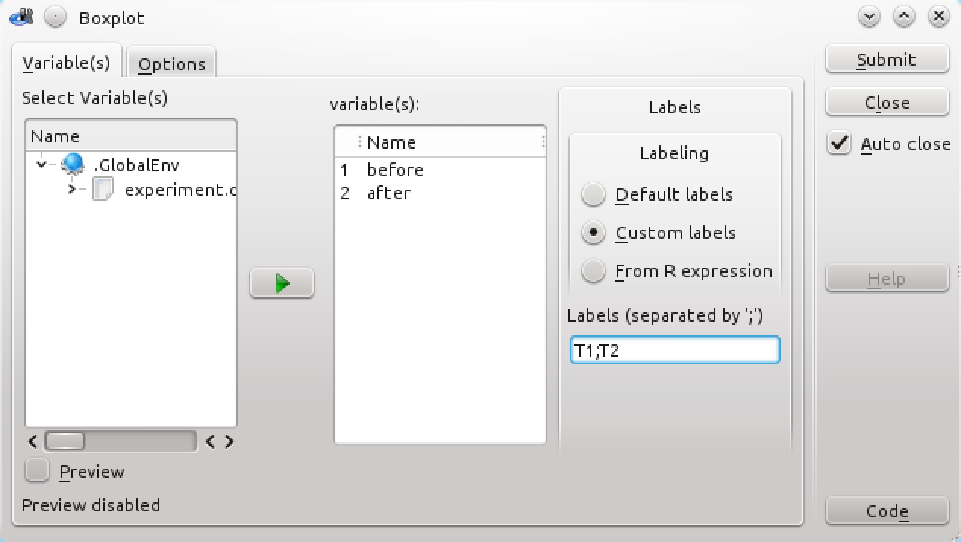
\includegraphics[width=15.5cm]{../figures/boxplot1.png}
 \caption{Boxplot dialog.}
 \label{fig:boxplot1}
\end{figure}

Checking the ``Preview'' box will open a graphics window, show the plot as
it is configured and update the window on changes in real time. From
that window it can be exported directly to several data formats as
well (Figure~\ref{fig:boxplot2}).

\begin{figure}[htp]
 \centering
 \includegraphics[width=15.5cm]{../figures/boxplot2.png}
 \caption{Plotted data and plot export dialog.}
 \label{fig:boxplot2}
\end{figure}

\section{Conclusion and outlook}
\label{sec:conclusion_summary}
In this article we have introduced the RKWard GUI to \proglang{R}. RKWard provides features ranging
from easy to use dialogs for common statistical procedures, targetted at \proglang{R} novices, to advanced
IDE features targetted at \proglang{R} experts.

Future versions of RKWard will continue to add value for both groups of users. Planned features include
an enhanced interface for debugging \proglang{R} code, support for editing more types of data, and the
ability to connect the RKWard GUI to a remote \proglang{R} engine. Perhaps most importantly, RKWard will
gain many new UI dialogs for manipulation, analysis, and visualization of data. The ability to
develop these dialogs as plugins allows any contributor or user to help in enhancing RKWard, without in-depth
programming knowledge.

\section{Acknowledgments}
\label{sec:acknowledgments}
The work described in this paper was supported by YOUR NAME OR THE NAME
OF SOMEBODELSE HERE

\bibliography{sources}
\end{document}
